\chapter{Controle e Alimentação}
\label{chapter:movimentacao}

\section{Carregador para bateria}

O carregador foi montado seguindo o esquema da Fig. \ref{fig:circuito_carregador.png}

\begin{figure}
    \begin{center}
        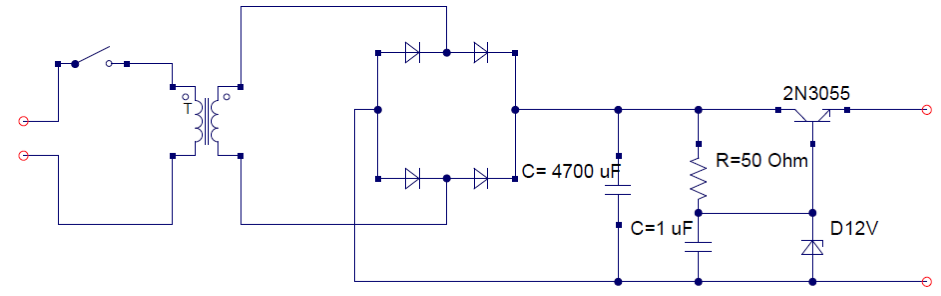
\includegraphics{figuras/circuito_carregador.png}
    \end{center}
    \caption{Circuito carregador da bateria}
    \label{fig:circuito_carregador.png}
\end{figure}

utilizando os seguintes materiais:

\begin{itemize}
    \item 1 transformador (entrada 110/220V, saída 15 V 5 A);
    \item 1 ponte retificadora 10A;
    \item fios vermelho e preto;
    \item 2 garras modelo “jacaré” (1 vermelho e 1 preto);
    \item 1 cabo de força;
    \item 1 fusível 10A;
    \item 1 porta fusível;
    \item 1 LED;
    \item 1 resistor de 1 k;
    \item botão de liga desliga e caixa de madeira;
    \item 1 capacitor de 4700 uF;
    \item 1 capacitor de 1uF;
    \item 1 transistor modelo 2N3055;
    \item 1 diodo zener de 15 V.
\end{itemize}

O transformador adquirido faz a transformação do valor de tensão RMS, dessa forma ao se converter a tensão alternada para contínua o valor de 15 V é multiplicado por $\sqrt{2}$. Como a tensão de carga da bateria é de aproximadamente 15 V, fez-se necessário a instalação de um circuito regulador de tensão.

Após a implementação do regulador de tensão foram feitos testes utilizando um multímetro para aferir a tensão de carga, como mostrado na Fig. \ref{fig:teste_carregador.png}

\begin{figure}
    \begin{center}
        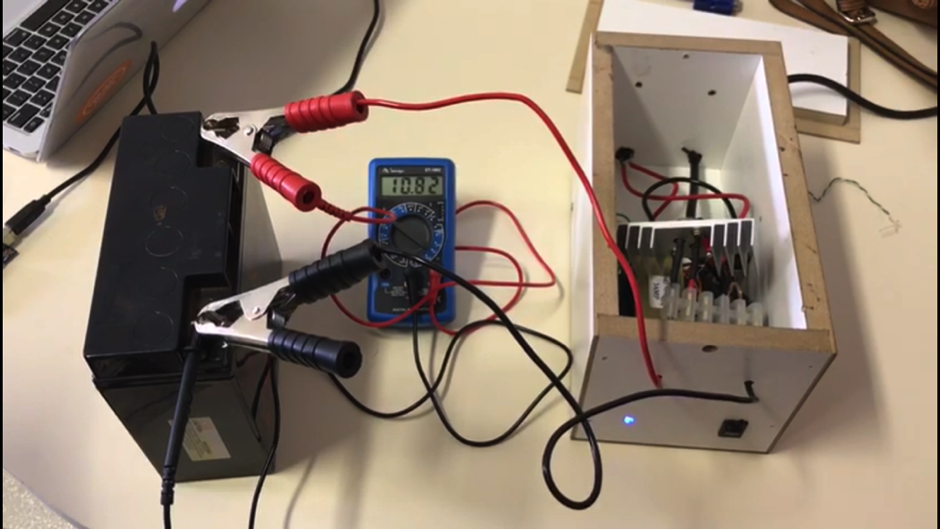
\includegraphics{figuras/teste_carregador.png}
    \end{center}
    \caption{Teste Carregador}
    \label{fig:teste_carregador.png}
\end{figure}

\section{Drive de Potência}

\subsection{Ponte H}

A ponte H do driver de potência foi fabricada em uma placa de circuito impresso de forma caseira. O layout foi feito utilizando o software Proteus. Como o circuito é projetado para alta potência, prestou-se atenção especial ao tamanho das trilhas , para garantir que a placa suportasse a quantidade de corrente que corre em suas trilhas. Dissipadores foram instalados nos MOSFETs conectados à fonte de alimentação dos motores, para assegurar que a temperatura dos mesmos não ultrapasse os valores limites. Para não ser necessário a re-soldagem dos transistores caso algum deles fosse danificado, foram adicionados soquetes que permitem a fácil retirada e instalação de novos transistores.

A Fig. \ref{fig:ponte_h.png} mostra a placa fabricada e utilizada na montagem final da cadeira

\begin{figure}
    \begin{center}
        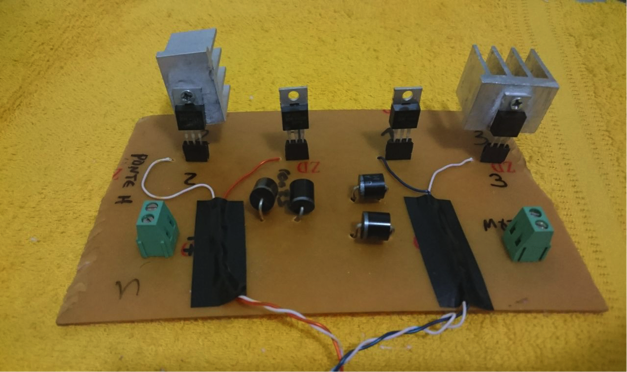
\includegraphics{figuras/ponte_h.png}
    \end{center}
    \caption{Circuito impresso ponte H.}
    \label{fig:ponte_h.png}
\end{figure}

\subsection{Circuito de chaveamento}

O projeto do circuito de chaveamento foi levemente alterado em relação ao mencionado no ponto de controle anterior. A funcionalidade permanece como antes, porém foi adicionado um circuito lógico combinacional utilizando portas AND (CI 7408) e inversora (CI 7404) na entrada para evitar a situação que aciona os dois lados da ponte H ao mesmo tempo, causando a queima total da ponte.

O circuito de chaveamento final foi realizado em protoboard e conectado com as outras partes do subsistema. A Fig. \ref{fig:circuito_chaveamento.png} mostra o circuito final:

\begin{figure}
    \begin{center}
        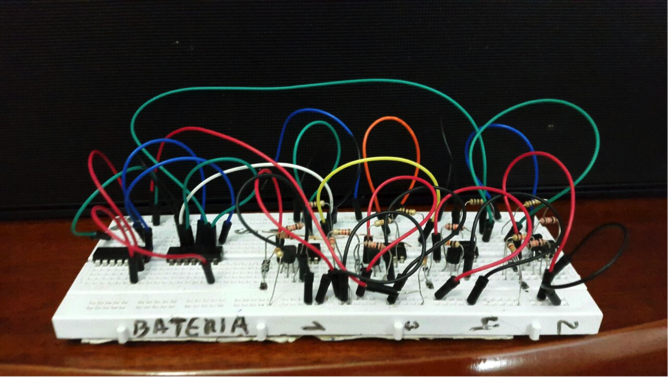
\includegraphics{figuras/circuito_chaveamento.png}
    \end{center}
    \caption{Circuito de chaveamento.}
    \label{fig:circuito_chaveamento.png}
\end{figure}

\subsection{Dobrador de tensão}

O circuito do dobrador de tensão foi feito em placa de circuito impresso de forma caseira e não houve alterações à partir da versão utilizada anteriormente. A Fig. \ref{fig:circuito_dobrador.png} mostra o circuito final do dobrador de tensão:

\begin{figure}
    \begin{center}
        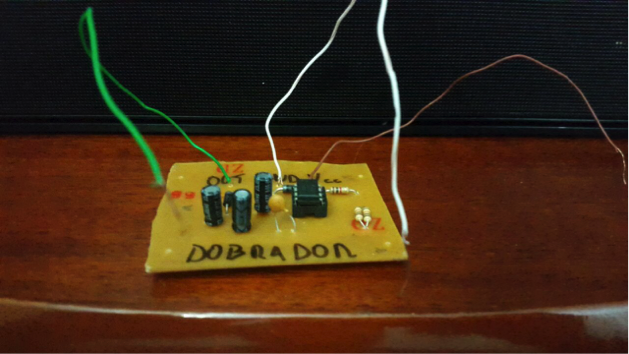
\includegraphics{figuras/circuito_dobrador.png}
    \end{center}
    \caption{Circuito impresso do dobrador de tensão.}
    \label{fig:circuito_dobrador.png}
\end{figure}

\section{Simulações}

A simulação do circuito completo com o dobrador de tensão, chaveamento e ponte H foi realizada utilizando o software Proteus e obteve-se resultados satisfatórios e que condizem com a realidade do projeto, realidade no que diz respeito a valores calculados para o funcionamento correto do circuito, tendo o motor seu sentido de giro de acordo com as entradas lidas pelo joystick. A simulação do circuito completo pode ser visto pela Fig. \ref{fig:simulacao.png} tendo o sentido do motor direcionado para a direita (sentido direto), em que o PWM tem uma frequência de 1 kHz e a entrada SENTIDO tem seu valor setado para nível lógico baixo.

\begin{figure}
    \begin{center}
        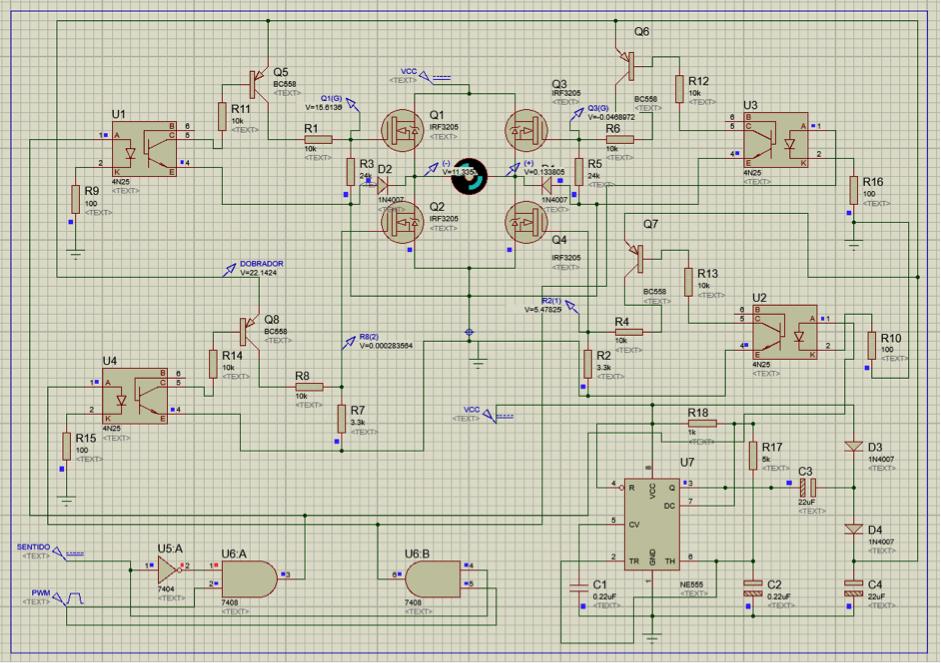
\includegraphics{figuras/simulacao.png}
    \end{center}
    \caption{Simulação do drive de potência.}
    \label{fig:simulacao.png}
\end{figure}

Diversas simulações utilizando o circuito foram realizadas para se ter a certeza de que os valores da entrada de cada transistor MOSFET da ponte H condizia com os valores calculados. Uma vez que estes valores eram iguais aos calculados, as confecções dos circuitos foram executadas como visto na seção anterior.

\section{Testes de Bancada}

Os testes de bancada podem ser vistos no Anexo X, onde os circuitos foram testados e avaliados segundo seu funcionamento. Os resultados de cada um dos testes foram satisfatórios, funcionando de acordo com o previsto.

\section{Integração}

Para a integração dos circuitos, construídos no subsistema de Controle e Alimentação, na cadeira de rodas, foi utilizado o esquema do circuito final da Fig. \ref{fig:circuito_integrado_cadeira.png}.

\begin{figure}
    \begin{center}
        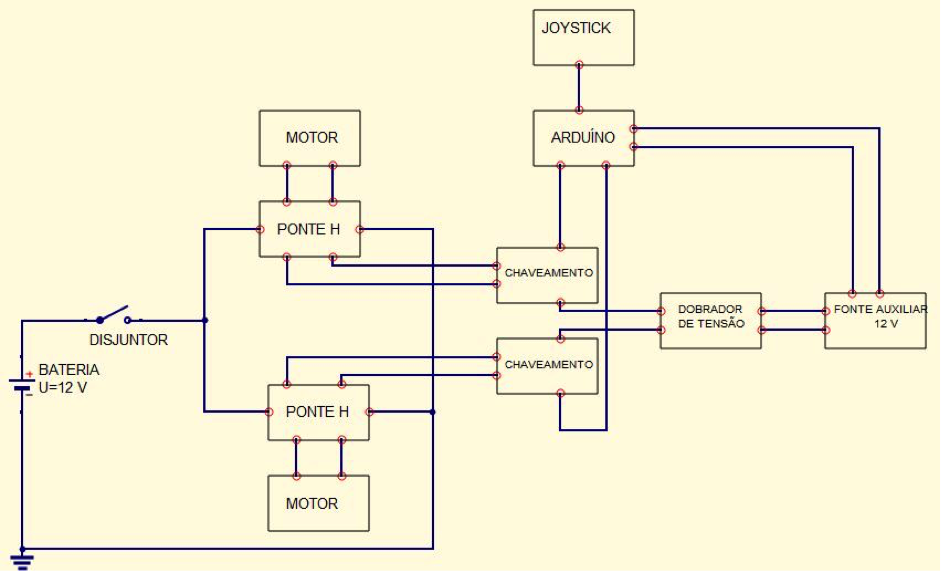
\includegraphics{figuras/circuito_integrado_cadeira.png}
    \end{center}
    \caption{Diagrama de integração do subsistema de controle e alimentação.}
    \label{fig:circuito_integrado_cadeira.png}
\end{figure}

Foi utilizado um disjuntor para o desligamento geral do circuito de alimentação, como forma de proteção do conjunto. A fonte auxiliar de 12 V foi conectada à um dobrador de tensão ligado aos chaveamentos, em que foram ligados ao arduino e joystick, e também ligados à ponte H e posteriormente ao motor. Foi feito o uso de uma bateria de 12 V para a alimentação dos componentes  de potência deste circuito.

Ao integrar o microcontrolador com o joystick ao circuito de chaveamento, ocorreu um erro que prejudica a solução final. Possivelmente por conta do número excessivo que o microcontrolador tem que alimentar, seu funcionamento fica prejudicado, fazendo com que seu ponto de referência ganhe um offset de aproximadamente 1.5V, fazendo com que seu nível lógico “baixo” não seja exatamente 0 volts, prejudicando assim a lógica combinacional que existe na entrada do circuito de chaveamento. Para solucionar este problema, foi projetado um circuito comparador, em uma tentativa de “forçar” o nível lógico baixo como 0 volts na saída do microcontrolador.

	Caso essa solução não apresente os resultados esperados, uma solução final para o problema será alterar a forma em que o usuário controla os movimentos da cadeira. Ao invés de utilizar o joystick, o mesmo e seu sistema de controle serão eliminados da versão final do projeto, sendo utilizado então botões analógicos para o controle do movimento da cadeira. Esta solução não é a ideal pois não permite o controle de velocidade dos motores, limitando o controle para apenas movimentos simples de “andar em frente”, “andar para trás” e “giro sobre o próprio eixo”. Outra limitação desta solução é o fato de que os motores estarão alimentados sempre em máxima potência alcançada pela ponte H (aproximadamente 80 por cento da potência máxima dos motores), possibilitando controles de arranque de partida e velocidades em geral.

